\documentclass[a4paper,11pt]{article}
%-----------
\usepackage{lipsum}
\usepackage{amssymb}
\usepackage{amsmath}
\usepackage{graphicx}
\usepackage{epstopdf}
\usepackage{placeins}
\usepackage{a4wide}
\usepackage[dutch]{babel}
\usepackage{multicol}
\usepackage[makeroom]{cancel}
\usepackage{enumerate}
\usepackage{lscape}
\usepackage{caption}
\usepackage[labelfont=bf]{caption}
\usepackage{hyperref}
%-----------
\usepackage{listings}
\renewcommand{\lstlistingname}{Matlab output}
%-----------
%\usepackage[utf8]{inputenc}
%\usepackage[T1]{fontenc}
%-----------
\title{Inleiding Programmeren: Opdracht 4}
\date{30-03-2019}
\author{Stoops Tom \\ 2 Ba Fysica}
%-----------
\newcommand{\paf}[3]{\frac{\partial^{#1} #2}{\partial #3^{#1}}}
%syntax: \partaf{A}{x} is partiele afgeleide van A naar x geevalueerd in x
\newcommand{\prop}[2]{s_{#2}^2\cdot\left(\paf{#1}{#2}\right)^2}
%syntax: analoog aan partaf, maar dan voor de propagatieformule (enkel sommeren erover en onder een wortel plaatsen: s_x = \sqrt{\prop{A}{a}+\prop{B}{b}+\ldots}
\renewcommand{\thefootnote}{\Roman{footnote}}
%\renewcommand{\phi}{\varphi}
\newcommand{\af}[3]{\frac{d^{#1}#2}{d {#3}^{#1}}}
%syntax: \af{4}{y}{x} is de 4de afgeleide van y naar x, voor 1ste afgeleide de eerste {} gewoon leeg laten!
\newcommand{\ste}{$^\mathrm{ste}\ $}
\newcommand{\de}{$^\mathrm{de}\ $}
%syntax: gewoon achter getal plaatsen
\newcommand{\p}[1]{\left(#1\right)}
\newcommand{\s}[1]{\left[#1\right]}
\newcommand{\avg}[1]{\left\langle#1\right\rangle}
\newcommand{\ta}{$\pm$}
\newcommand{\cirkel}[1]{\raisebox{.5pt}{\textcircled{\raisebox{-1.1pt} {#1}}}}
\let\oldexp\exp
\renewcommand{\exp}[1]{\oldexp\p{#1}}
\newcommand{\exps}[1]{\oldexp\s{#1}}
\newcommand{\abs}[1]{\left|#1\right|}
%-----------
%\captionsetup{width=0.8\textwidth}
%-----------
\begin{document}
\pagenumbering{arabic}
\maketitle

\begin{flushright}
  \textsl{Voor ruwe console output, zie \texttt{OUTPUT\_CONSOLE.TXT}.}
\end{flushright}

\section*{Theorie}
  \noindent
  In deze taak zullen we de eendimensionale diffusie vergelijking oplossen, algemeen gegeven door:
  \begin{equation}
    \paf{2}{}{x}T\p{x,t}-\frac1\kappa\paf{}{}{t}T\p{x,t} = 0
  \end{equation}
  Hiervoor zullen we volgend explicit finite difference \cite{NM} discretisatieschema gebruiken:\footnote{Ook gegeven in de opdracht.}
  \begin{equation}
    T_{i,j+1} = T_{i,j}+\eta\p{T_{i+1,j}+T_{i-1,j}-2T_{i,j}}
  \end{equation}
  Waar $i$ de ruimtestap is en $j$ de tijdstap. Hier is $\eta$ een constante die overeenkomt met de Courant-Friedrichs-Levy voorwaarde op stabiliteit die bepaald wordt met behulp van Von Neumann stabiliteitsanalyse. Hiervoor is in de opdracht gegeven dat deze voorwaarde gegeven is door:
  \begin{equation}
    \eta = \frac{K\Delta t}{C\rho\p{\Delta x}^2} < \frac12
    \label{stabiliteit}
  \end{equation}

  \noindent
  In deze opdracht zullen we ook twee vormen van randvoorwaarden beschouwen. Ten eerste de Dirichlet randvoorwaarde, die zeggen dat:
  \begin{equation}
    \left\{
    \begin{align}
      T\p{0,t} &= \alpha \\
      T\p{L,t} &= \beta
    \end{align}
    \right. \qquad\text{met } \alpha,\beta\in\mathbb{R}
  \end{equation}
  Waarbij de randpunten dus een constante waarde toegewezen krijgen. Ten tweede Neumann randvoorwaarden, gegeven door:
  \begin{equation}
    \left\{
    \begin{align}
      \paf{}{}{x}T\p{0,t} &= \gamma \\
      \paf{}{}{x}T\p{L,t} &= \delta
    \end{align}
    \right. \qquad\text{met } \gamma,\delta\in\mathbb{R}
  \end{equation}
  Waarbij dus de afgeleiden op de randpunten constant blijven.

\newpage
\section*{Taak 1}
  \FloatBarrier
  \begin{figure}[ht!]
    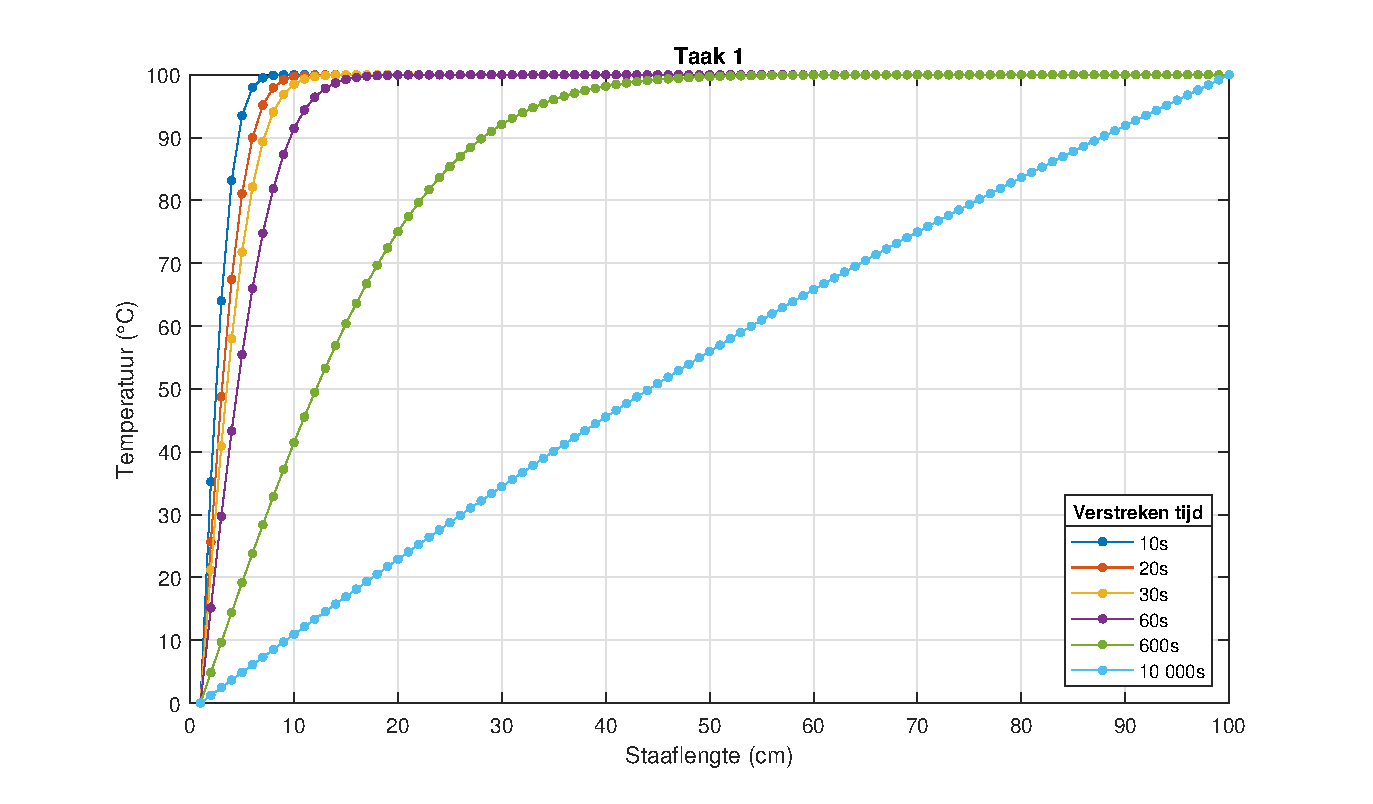
\includegraphics[width = \textwidth]{taak1.eps}
    \caption{Gevonden temperatuursverdeling op verschillende tijdstippen voor taak 1.}
    \label{taak1}
  \end{figure}
  \FloatBarrier

  \noindent
  We zien voor de diffusie van temperatuur bij Dirichlet randvoorwaarden met beginvoorwaarde dat de gehele staaf\footnote{Op het linkse randpunt na.} op 100 $^\circ$C naar een (bij benadering) lineaire stijging convergeert na verloop van voldoende tijd. Dit is heel duidelijk op de grafiek voor $t$ = 10 000 s.\\

  \noindent
  Dit is ook een logisch gegeven als we naar een relaxatie-methode zouden kijken voor dit probleem, hierbij wordt bij iedere iteratie het gemiddelde genomen tussen de naburige punten waardoor we een rechte met voorschrift $T = \frac{100\ ^\circ\mathrm{C}}{100 \ \mathrm{cm}}\cdot L$.

\newpage
\section*{Taak 2}
  \FloatBarrier
  \begin{figure}[ht!]
    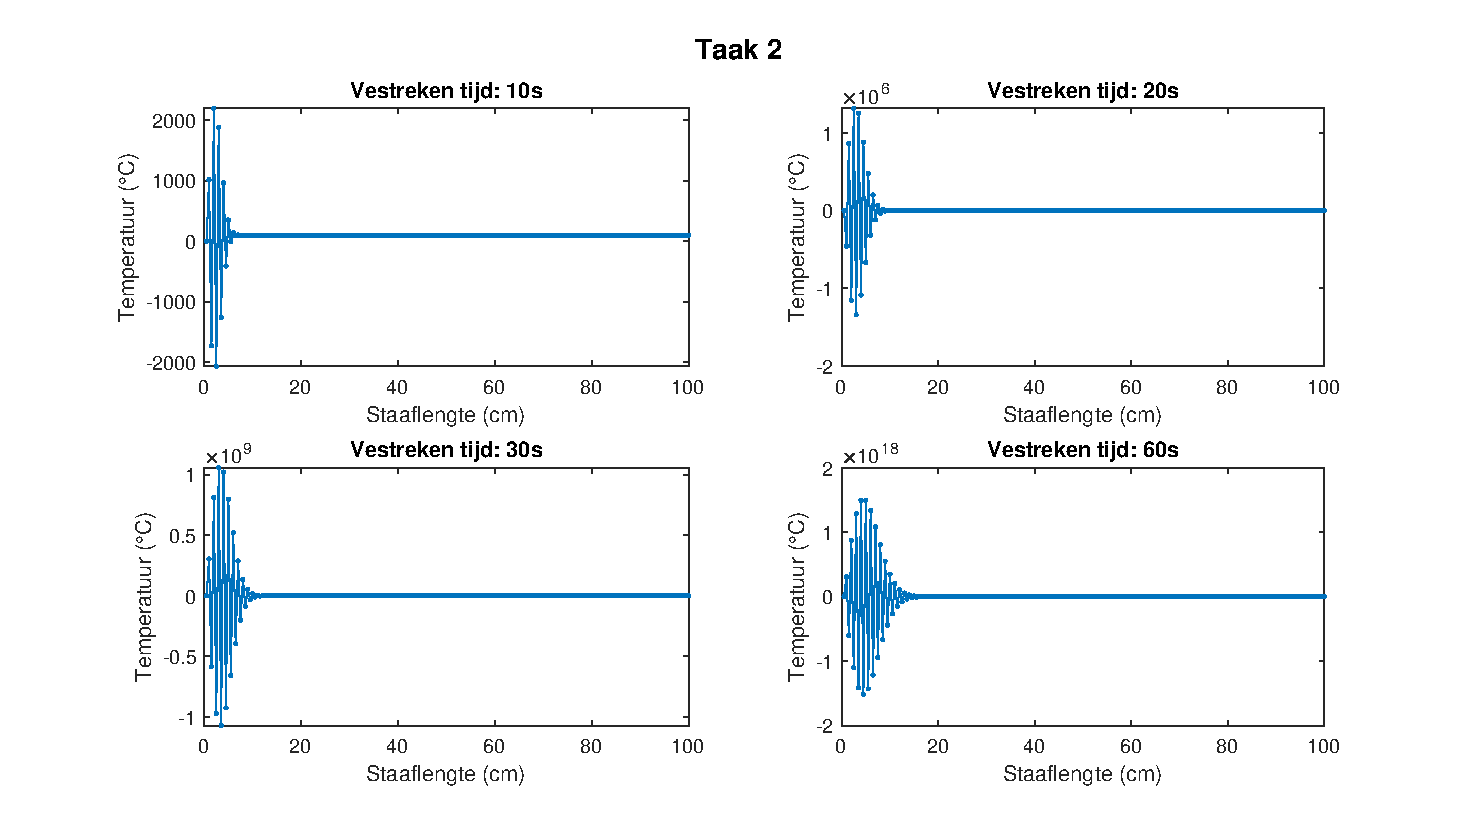
\includegraphics[width = \textwidth]{taak2.eps}
    \caption{Gevonden temperatuursverdeling op verschillende tijdstippen voor taak 2.}
    \label{taak2}
  \end{figure}
  \FloatBarrier

  \noindent
  Wanneer er niet voldaan is aan het stabiliteitscriterium \eqref{stabiliteit} vinden we dat de resultaten divergeren van de oplossing. We zien op figuur \ref{taak2} duidelijk dat de instabiliteit en fout op het juiste antwoord enorm snel groeit. Als het algoritme instabiel is kunnen we hier geen correcte oplossing uit verwachten. Voor tijdstap $t$ = 600 s gaf \texttt{C++} zelfs \texttt{-nan(ind)} terug als waarde wegens overflow van waarden.

\newpage
\section*{Taak 3}
  \FloatBarrier
  \begin{figure}[ht!]
    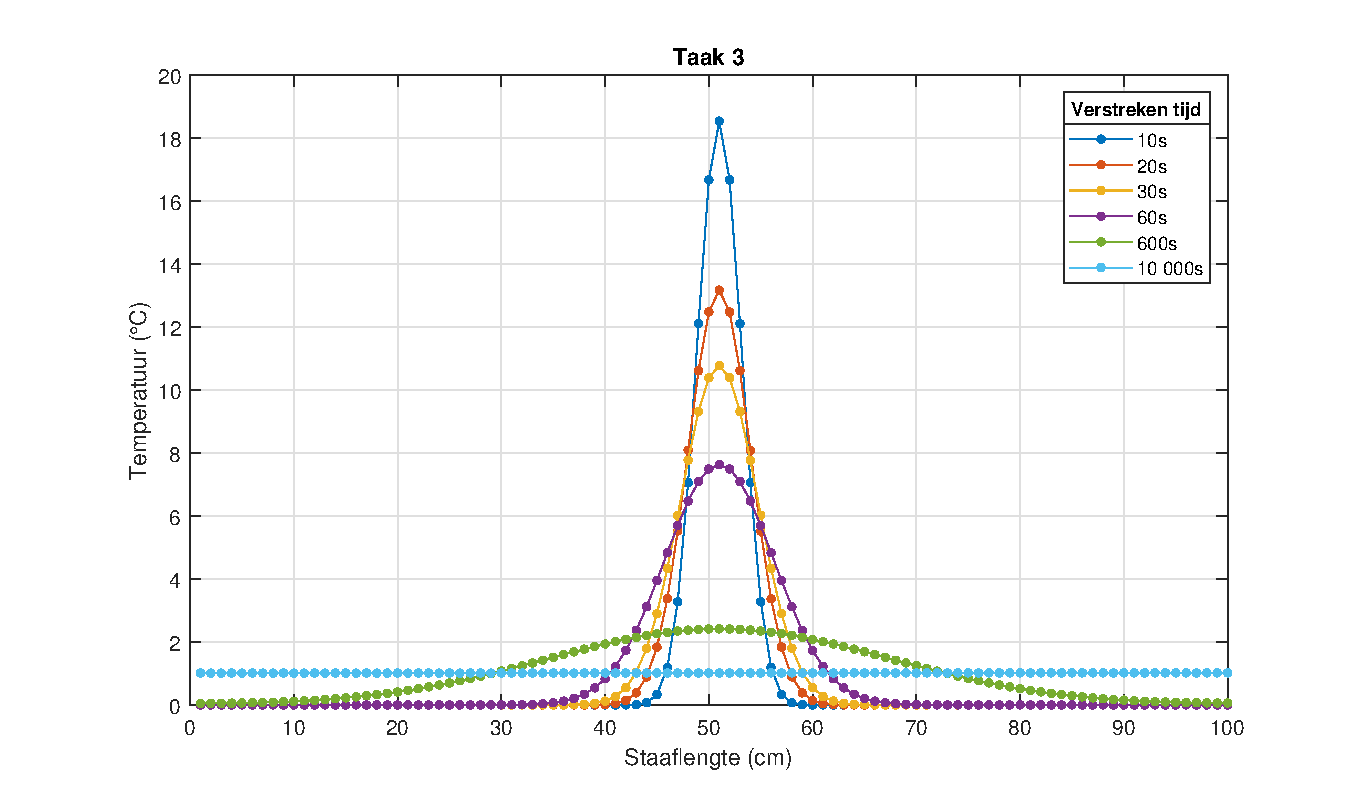
\includegraphics[width = \textwidth]{taak3.eps}
    \caption{Gevonden temperatuursverdeling op verschillende tijdstippen voor taak 3.}
    \label{taak3}
  \end{figure}
  \FloatBarrier

  \noindent
  In deze taak werd de beginvoorwaarde gegeven door een delta piek in het midden van de staaf met Neumann randvoorwaarden. We zien hier dat de initi\"ele piek al snel uitdijnt tot een Gauss-achtige curve waarvan de $\sigma$-waarde steeds toeneemt. Na lange tijd ($t$ = 10 000 s) zien we dat de staaf op een vrijwel homogeen verdeelde temperatuur is gekomen van 1 $^\circ$C.

\begin{thebibliography}{99}
  \bibitem{NM} M. Milo\v{s}evi\'c \textit{Cursus: Numerical Methods}, UAntwerpen
\end{thebibliography}
\end{document}
